% !TeX program = xelatex
% !BIB program = biber
\documentclass[light]{lutbeamer}

\usepackage{pgfpages}
\usepackage{ragged2e}
\usepackage{booktabs}
\usepackage{amssymb}
\usepackage{fontawesome5}
\usepackage{tikz}
\usepackage{pgfplots}
\pgfplotsset{compat=1.18}
\addbibresource{references.bib}

% ===================================================================
% METADATA
% ===================================================================
\setdepartment{OSTİM Teknik Üniversitesi}
\institute{}
\author[Mühendislik Fakültesi]{\\
Prof.~Dr.~Yalçın ATA \\
Prof.~Dr.~Arif DEMİR \\
Dr.~Öğr.~Üyesi~Muhammed ELMNEFİ \\
Dr.~Öğr.~Üyesi~Haydar KILIÇ \\
Dr.~Öğr.~Üyesi~Emel GÜVEN \\
Dr.~Öğr.~Üyesi~Ufuk ASIL \\
Öğr.~Gör.~Sema ÇİFTÇİ
}
\title{MATH 204 -- Olasılık ve İstatistik}
\subtitle{Hafta 10: Sürekli Olasılık Dağılımları}
\date{2025--2026 Bahar Dönemi}

% ===================================================================
% OTOMATİK İÇİNDEKİLER
% ===================================================================
\setcounter{tocdepth}{2}

\AtBeginSection[]{
  \begin{frame}{Sunum Planı}
    \scriptsize
    \begin{columns}[T]
      \begin{column}{0.48\textwidth}
        \tableofcontents[sections={1-3}, currentsection]
      \end{column}
      \begin{column}{0.48\textwidth}
        \tableofcontents[sections={4-10}, currentsection]
      \end{column}
    \end{columns}
  \end{frame}
}

\begin{document}

\setbeamertemplate{navigation symbols}{}
\setbeamertemplate{footline}{
  \begin{beamercolorbox}[wd=\paperwidth, ht=10pt, dp=1pt]{footline}
    \usebeamerfont{footline}
    \begin{tikzpicture}[remember picture,overlay]
      \node[anchor=south west, xshift=10mm, yshift=.4mm]
      at (current page.south west)
      {\insertshortauthor,~\department};
    \end{tikzpicture}
    \begin{tikzpicture}[remember picture,overlay]
      \node[anchor=south east, xshift=-5mm, yshift=0.5mm]
      at (current page.south east)
      {\insertframenumber \,/\, \inserttotalframenumber};
    \end{tikzpicture}
  \end{beamercolorbox}
}

% ===================================================================
% KAPAK
% ===================================================================
\begin{frame}<article:0>[plain,noframenumbering]
  \begin{tikzpicture}[remember picture,overlay]
    \node[anchor=center, at=(current page.center), inner sep=0pt] {
      \includegraphics[width=\paperwidth, height=\paperheight]{logos/background_figure.jpg}
    };
  \end{tikzpicture}
\end{frame}

{
  \setbeamertemplate{footline}{
    \begin{beamercolorbox}[wd=\paperwidth, ht=10pt, dp=1pt]{footline}
      \usebeamerfont{footline}
      \begin{tikzpicture}[remember picture,overlay]
        \node[anchor=south west, xshift=10mm, yshift=.4mm, align=left]
        at (current page.south west)
        {\tiny Bu şablon OTÜ Yazılım Mühendisliği tarafından hazırlanmış olup \href{https://github.com/ufukasia/Ostim-Teknik--niversitesi-Yaz-l-m-M-hendisli-i---Lutbeamer-egitim-i-eri-i-haz-rlama-}{buradan} güncel haline ulaşabilirsiniz.};
      \end{tikzpicture}
      \begin{tikzpicture}[remember picture,overlay]
        \node[anchor=south east, xshift=-5mm, yshift=0.5mm]
        at (current page.south east)
        {\insertframenumber \,/\, \inserttotalframenumber};
      \end{tikzpicture}
    \end{beamercolorbox}
  }
  \setbeamerfont{title}{size=\large}
  \setbeamerfont{author}{size=\scriptsize}
  \setbeamerfont{subtitle}{size=\small}
  \setbeamerfont{date}{size=\footnotesize}
  \maketitle{}
}

\begin{frame}{İçindekiler}
  \scriptsize
  \begin{columns}[T]
    \begin{column}{0.48\textwidth}
      \tableofcontents[sections={1-3}]
    \end{column}
    \begin{column}{0.48\textwidth}
      \tableofcontents[sections={4-10}]
    \end{column}
  \end{columns}
\end{frame}

% ===================================================================
% SECTION 1
% ===================================================================
\section{Hafta 9'dan Bu Haftaya}
\subsection{Hatırlatma ve Yön}

\begin{frame}{Hafta 9'dan Ne Getiriyoruz?}
    \small
    \begin{block}{Elimizdeki ayrık dil}
        Geçen hafta şu aileleri tanıdık:
        \[
        \text{Binom},\ \text{Hipergeometrik},\ \text{Geometrik},\ \text{Negatif Binom},\ \text{Poisson}.
        \]
    \end{block}

    \begin{itemize}
        \item Hepsi \textbf{sayılabilir değerler} alan rastgele değişkenler üretiyordu.
        \item Olasılıkları çoğu zaman \textbf{tek tek noktalara} atayabiliyorduk.
        \item Şimdi odağımız değişiyor: ölçüm, tolerans, süre ve ömür gibi büyüklükler \textbf{aralıklar} üzerinde düşünülüyor.
    \end{itemize}

    \begin{alertblock}{Bu haftanın sorusu}
        Saydığımız şeyi değil, \textbf{ölçtüğümüz büyüklüğün dağılım biçimini} nasıl okuyacağız?
    \end{alertblock}
\end{frame}

\begin{frame}{Kavram Haritası: Sürekli Dağılım Aileleri}
    \centering
    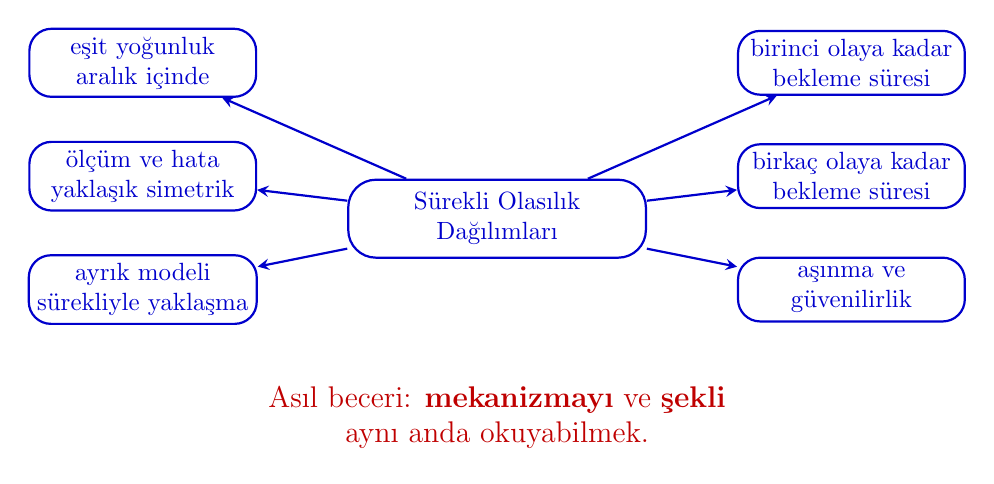
\begin{tikzpicture}[>=stealth, thick, scale=0.9, transform shape]
        \colorlet{myblue}{blue!80!black}
        \colorlet{myred}{red!75!black}

        \node[draw=myblue, rounded corners=10pt, minimum width=4.2cm, minimum height=1.1cm, text=myblue, align=center] (root) at (0,0) {Sürekli Olasılık\\Dağılımları};

        \node[draw=myblue, rounded corners=8pt, minimum width=3.2cm, minimum height=0.9cm, text=myblue, align=center] (uniform) at (-5,2.2) {eşit yoğunluk\\aralık içinde};
        \node[draw=myblue, rounded corners=8pt, minimum width=3.2cm, minimum height=0.9cm, text=myblue, align=center] (normal) at (-5,0.6) {ölçüm ve hata\\yaklaşık simetrik};
        \node[draw=myblue, rounded corners=8pt, minimum width=3.2cm, minimum height=0.9cm, text=myblue, align=center] (approx) at (-5,-1.0) {ayrık modeli\\sürekliyle yaklaşma};
        \node[draw=myblue, rounded corners=8pt, minimum width=3.2cm, minimum height=0.9cm, text=myblue, align=center] (expo) at (5,2.2) {birinci olaya kadar\\bekleme süresi};
        \node[draw=myblue, rounded corners=8pt, minimum width=3.2cm, minimum height=0.9cm, text=myblue, align=center] (gamma) at (5,0.6) {birkaç olaya kadar\\bekleme süresi};
        \node[draw=myblue, rounded corners=8pt, minimum width=3.2cm, minimum height=0.9cm, text=myblue, align=center] (weibull) at (5,-1.0) {aşınma ve\\güvenilirlik};

        \draw[->, myblue] (root) -- (uniform);
        \draw[->, myblue] (root) -- (normal);
        \draw[->, myblue] (root) -- (approx);
        \draw[->, myblue] (root) -- (expo);
        \draw[->, myblue] (root) -- (gamma);
        \draw[->, myblue] (root) -- (weibull);

        \node[text=myred, font=\large, align=center] at (0,-2.8) {Asıl beceri: \textbf{mekanizmayı} ve \textbf{şekli}\\ aynı anda okuyabilmek.};
    \end{tikzpicture}
\end{frame}

\begin{frame}{Neden Tek Bir PDF Yetmez?}
    \small
    \begin{columns}[T]
        \begin{column}{0.48\textwidth}
            \begin{block}{Farklı süreçler, farklı şekiller}
                \begin{itemize}
                    \item Toplantı süresi sınırlı bir aralıkta olabilir.
                    \item Ölçüm hataları çoğu kez merkezin çevresinde kümelenir.
                    \item İlk arızaya kadar geçen süre sağa çarpık olabilir.
                    \item Aşınan mekanik parçalarda arıza riski yaşla birlikte artabilir.
                \end{itemize}
            \end{block}
        \end{column}
        \begin{column}{0.48\textwidth}
            \begin{alertblock}{Sonuç}
                Tek bir sürekli yoğunluk fonksiyonu bütün süreçlere uymaz.
                Önce sürecin \textbf{doğasını}, sonra da yoğunluğun \textbf{şeklini} okuruz.
            \end{alertblock}

            \vspace{0.3cm}
            \begin{itemize}
                \item Sınır var mı?
                \item Simetri var mı?
                \item Bekleme mi sayıyoruz?
                \item Arıza riski zamanla sabit mi?
            \end{itemize}
        \end{column}
    \end{columns}
\end{frame}

\begin{frame}{Bu Haftanın Öğrenme Hedefleri}
    \small
    \begin{enumerate}
        \item Sürekli uniform, normal, üssel, gamma ve Weibull ailelerinin \textbf{ne zaman uygun} olduğunu ayırt etmek.
        \item Sürekli bir değişkende olasılığın \textbf{nokta değil aralık} üzerinden hesaplandığını netleştirmek.
        \item Normal dağılımda \textbf{z-dönüşümü} kullanarak tablo okuması yapmak.
        \item Binom dağılımı için \textbf{normal yaklaşım} ve \textbf{süreklilik düzeltmesini} yorumlamak.
        \item Bekleme süresi ve güvenilirlik problemlerinde \textbf{üssel-gamma-Weibull} farkını okumak.
    \end{enumerate}

    \begin{exampleblock}{Dersin tek cümlelik çıktısı}
        Sürekli bir problemi yalnız formülle değil, \textbf{dağılım ailesi + parametre yorumu + süreç mantığı} ile çözeceğiz.
    \end{exampleblock}
\end{frame}

\begin{frame}{Model Seçme Sorusu: Hangi Süreç Hangi Aileyi Çağırır?}
    \scriptsize
    \begin{center}
        \resizebox{0.97\textwidth}{!}{
        \begin{tabular}{@{}lll@{}}
            \toprule
            \textbf{Problem cümlesi} & \textbf{Ana ipucu} & \textbf{Doğal aday} \\ \midrule
            Bir sürenin sadece \([A,B]\) aralığında olması & her nokta eşit yoğunlukta & sürekli uniform \\
            Ölçüm hatası / üretim çapı / sınav skoru & simetrik merkez etrafında yayılım & normal \\
            Büyük \(n\), uygun \(p\) için binom hesabı & ayrığı sürekliyle yaklaşma & normal yaklaşım \\
            İlk çağrıya kadar geçen süre & Poisson sürecinde birinci olay & üssel \\
            \(k\). olaya kadar geçen süre & birden çok olayı bekleme & gamma \\
            Aşınan mekanik parçada ömür & arıza riski sabit değil & Weibull \\ \bottomrule
        \end{tabular}}
    \end{center}

    \begin{alertblock}{Refleks}
        Önce şu soruyu sorun:
        \textbf{``Bu büyüklüğün şekli ve üretim mekanizması bana ne söylüyor?''}
    \end{alertblock}
\end{frame}

\begin{frame}{Isınma: PDF, CDF ve Sürekli Olasılık Dili}
    \small
    \begin{block}{Temel fark}
        Sürekli bir rastgele değişkende
        \[
        P(X=x)=0
        \]
        olur. Olasılıkları aralıklar üzerinden okuruz.
    \end{block}

    \begin{columns}[T]
        \begin{column}{0.48\textwidth}
            \begin{itemize}
                \item \textbf{PDF} \(f(x)\): yoğunluğu anlatır.
                \item \textbf{CDF} \(F(x)=P(X\le x)\): birikimli olasılığı verir.
                \item \textbf{Aralık olasılığı}:
                \[
                P(a<X<b)=\int_a^b f(x)\,dx.
                \]
            \end{itemize}
        \end{column}
        \begin{column}{0.48\textwidth}
            \begin{alertblock}{Kritik sezgi}
                Sürekli modelde \textbf{yükseklik} olasılık değildir;
                \textbf{alan} olasılıktır.
            \end{alertblock}
        \end{column}
    \end{columns}
\end{frame}

% ===================================================================
% SECTION 2
% ===================================================================
\section{Sürekli Uniform Dağılım (Bölüm 6.1)}
\subsection{Eşit Yoğunluk Fikri}

\begin{frame}{Eşit Olasılık Değil, Eşit Yoğunluk}
    \small
    \begin{block}{Sürekli uniform sezgisi}
        Bir büyüklük yalnızca \([A,B]\) aralığında değer alıyor ve aralık içinde
        her nokta \textbf{aynı yoğunlukla} temsil ediliyorsa sürekli uniform düşünürüz.
    \end{block}

    \begin{itemize}
        \item Bu, ayrık uniformdaki gibi ``her tek değerin olasılığı eşit'' demek değildir.
        \item Asıl fikir: \textbf{eşit uzunluklu alt aralıklar eşit olasılık taşır}.
        \item Grafik, yüksekliği sabit bir dikdörtgendir.
    \end{itemize}

    \begin{alertblock}{Örnek bağlam}
        Toplantı süresi, geliş zamanı, ölçüm gecikmesi veya döngü içindeki rastgele faz konumu.
    \end{alertblock}
\end{frame}

\begin{frame}{Dikdörtgen Yoğunluk: \(U(A,B)\)}
    \small
    \(X \sim U(A,B)\) için yoğunluk fonksiyonu
    \[
    f(x)=
    \begin{cases}
    \dfrac{1}{B-A}, & A \le x \le B,\\
    0, & \text{aksi halde}.
    \end{cases}
    \]

    \begin{columns}[T]
        \begin{column}{0.48\textwidth}
            \begin{itemize}
                \item Yükseklik sabittir.
                \item Toplam alan \(1\) olmalıdır.
                \item Bu yüzden yükseklik otomatik olarak \(1/(B-A)\) çıkar.
            \end{itemize}
        \end{column}
        \begin{column}{0.48\textwidth}
            \begin{exampleblock}{Kısa kontrol}
                \[
                \int_A^B \frac{1}{B-A}\,dx=1.
                \]
                Yani model gerçekten bir yoğunluk fonksiyonudur.
            \end{exampleblock}
        \end{column}
    \end{columns}
\end{frame}

\begin{frame}{Olasılık Neden Uzunluk ile Hesaplanır?}
    \small
    Uniform dağılımda aralık olasılığı basitçe dikdörtgen alanıdır:
    \[
    P(a<X<b)=\frac{b-a}{B-A}, \qquad A\le a<b \le B.
    \]

    \begin{block}{Yorum}
        Uniform dağılımda olasılık, tüm aralığın ne kadarını kapladığınıza bağlıdır.
    \end{block}

    \begin{exampleblock}{Hızlı okuma}
        Eğer \(X \sim U(0,4)\) ise
        \[
        P(1<X<3)=\frac{3-1}{4-0}=\frac{1}{2}.
        \]
    \end{exampleblock}
\end{frame}

\begin{frame}{Örnek 1: Toplantı Süresi 0 ile 4 Saat Arasında}
    \small
    Bir proje toplantısının süresi \(X\) saat cinsinden ölçülüyor ve
    \[
    X \sim U(0,4)
    \]
    kabul ediliyor.

    \begin{enumerate}
        \item Toplantının \(1\) saatten uzun sürme olasılığı nedir?
        \item Toplantının \(1\) ile \(2.5\) saat arasında sürme olasılığı nedir?
    \end{enumerate}

    \[
    P(X>1)=\frac{4-1}{4}=0.75
    \]
    \[
    P(1<X<2.5)=\frac{2.5-1}{4}=0.375
    \]
\end{frame}

\begin{frame}{Örnek 2: Sensör Gecikmesi 2 ile 5 ms Arasında}
    \small
    Bir sensörün tepki gecikmesi \(X\) milisaniye cinsinden
    \[
    X \sim U(2,5)
    \]
    ile modelleniyor.

    \begin{block}{Soru}
        Gecikmenin \(4\) ms'den büyük olma olasılığı nedir?
    \end{block}

    \[
    P(X>4)=\frac{5-4}{5-2}=\frac{1}{3}\approx 0.333.
    \]

    \begin{alertblock}{Yorum}
        Aralığın son üçte birlik kısmına girdiğimiz için olasılık da üçte birdir.
    \end{alertblock}
\end{frame}

\begin{frame}{Ortalama ve Varyans: Uniformun Merkezi}
    \small
    Sürekli uniform dağılım için
    \[
    E(X)=\frac{A+B}{2}, \qquad \mathrm{Var}(X)=\frac{(B-A)^2}{12}.
    \]

    \begin{columns}[T]
        \begin{column}{0.48\textwidth}
            \begin{block}{Sezgi}
                \begin{itemize}
                    \item Ortalama tam orta noktadır.
                    \item Yayılım aralığın genişliği ile büyür.
                    \item Aralık iki katına çıkarsa varyans dört katına çıkar.
                \end{itemize}
            \end{block}
        \end{column}
        \begin{column}{0.48\textwidth}
            \begin{exampleblock}{Kısa hesap}
                Eğer \(X \sim U(2,5)\) ise
                \[
                E(X)=3.5
                \]
                \[
                \mathrm{Var}(X)=\frac{9}{12}=0.75.
                \]
            \end{exampleblock}
        \end{column}
    \end{columns}
\end{frame}

\begin{frame}{Uniform Sorularında Sık Hata}
    \small
    \begin{enumerate}
        \item Yoğunluk yüksekliğini doğrudan olasılık sanmak
        \item Aralık dışındaki değerler için pozitif olasılık yazmak
        \item Nokta olasılığını sıfır yerine ``çok küçük'' gibi okumak
        \item Sürecin gerçekten eşit yoğunluk varsayımını destekleyip desteklemediğini sorgulamamak
    \end{enumerate}

    \begin{alertblock}{Kontrol listesi}
        \begin{itemize}
            \item Aralık net mi?
            \item Yoğunluk sabit mi?
            \item İstenen şey bir nokta mı, aralık mı?
        \end{itemize}
    \end{alertblock}
\end{frame}

\subsection{Pekiştirme Sorusu}

\begin{frame}{Soru 1: Boya Kuruma Süresi}
    \small
    Bir endüstriyel boyanın kuruma süresi \(X\) dakika cinsinden
    \[
    X \sim U(30,50)
    \]
    ile modelleniyor.

    \begin{enumerate}
        \item[(a)] Kuruma süresinin \(34\) ile \(42\) dakika arasında olma olasılığı nedir?
        \item[(b)] Beklenen kuruma süresi kaç dakikadır?
    \end{enumerate}
\end{frame}

\begin{frame}{Soru 1: Çözüm İçin Durak}
    \color{red!70!black}
    \small
    \[
    P(34<X<42)=\frac{42-34}{50-30}
    \]
    \[
    E(X)=\frac{30+50}{2}
    \]

    \begin{center}
        \textit{Uniform dağılımda olasılık, ilgili alt aralığın toplam aralığa oranıdır.}
    \end{center}
\end{frame}

\begin{frame}{Soru 1: Çözüm}
    \small
    \[
    P(34<X<42)=\frac{8}{20}=0.40.
    \]

    \[
    E(X)=40 \text{ dakika}.
    \]

    \begin{exampleblock}{Yorum}
        Model bu boyanın ortalama \(40\) dakikada kuruduğunu, \(34\) ile \(42\) dakika arasında kuruma olasılığının ise \(\%40\) olduğunu söylüyor.
    \end{exampleblock}
\end{frame}

\section{Normal Dağılım ve Normal Eğri (Bölüm 6.2--6.4)}
\subsection{Şekil ve Parametreler}

\begin{frame}{Neden Normal Eğri Bu Kadar Merkezi?}
    \small
    Normal dağılım; ölçüm hataları, üretim toleransları, biyolojik değişkenlik ve çok sayıda küçük etkinin toplamı gibi durumlarda sık görülür.

    \begin{itemize}
        \item Merkez etrafında yoğunlaşma vardır.
        \item Sağ ve sol kuyruk simetriktir.
        \item Büyük sapmalar mümkündür ama seyrektir.
    \end{itemize}

    \begin{alertblock}{Mühendislik okuması}
        Tornalanmış parça çapı, sensör ölçüm hatası veya sınav performansı gibi değişkenler sıklıkla normal modelle yaklaşık açıklanır.
    \end{alertblock}
\end{frame}

\begin{frame}{Normal Yoğunluk Fonksiyonu}
    \small
    \(X \sim N(\mu,\sigma^2)\) için yoğunluk
    \[
    f(x)=\frac{1}{\sigma\sqrt{2\pi}}
    e^{-\frac{1}{2}\left(\frac{x-\mu}{\sigma}\right)^2},
    \qquad -\infty < x < \infty
    \]
    biçimindedir.

    \begin{block}{Parametreler}
        \begin{itemize}
            \item \(\mu\): merkez
            \item \(\sigma\): standart sapma, yani yayılım ölçeği
        \end{itemize}
    \end{block}

    \begin{alertblock}{Kritik bilgi}
        Eğrinin toplam alanı \(1\)'dir; olasılık yine alanla hesaplanır.
    \end{alertblock}
\end{frame}

\begin{frame}{Parametrelerin Rolü: \(\mu\) Kaydırır, \(\sigma\) Yaydırır}
    \small
    \begin{columns}[T]
        \begin{column}{0.48\textwidth}
            \begin{block}{\(\mu\) değişirse}
                Eğrinin biçimi aynı kalır, sadece merkez sağa ya da sola kayar.
            \end{block}

            \[
            N(50,5^2) \quad \text{ve} \quad N(60,5^2)
            \]
            aynı genişlikte, farklı merkezde iki eğridir.
        \end{column}
        \begin{column}{0.48\textwidth}
            \begin{block}{\(\sigma\) değişirse}
                Merkez sabit kalsa bile eğri daralır ya da yayılır.
            \end{block}

            \[
            N(50,3^2) \quad \text{ve} \quad N(50,8^2)
            \]
            aynı merkezde, farklı yayılıma sahip iki eğridir.
        \end{column}
    \end{columns}
\end{frame}

\begin{frame}{Normal Eğrinin Temel Özellikleri}
    \small
    \begin{enumerate}
        \item Eğri simetriktir.
        \item Ortalama, medyan ve mod aynı noktadadır.
        \item Kuyruklar yatay eksene asimptotik yaklaşır.
        \item Toplam alan \(1\)'dir.
        \item Eğrinin dönüm noktaları yaklaşık \(\mu \pm \sigma\) civarındadır.
    \end{enumerate}

    \begin{exampleblock}{Neden önemli?}
        Bu özellikler hem tablo kullanımını hem de veri yorumunu kolaylaştırır.
    \end{exampleblock}
\end{frame}

\begin{frame}{Örnek 3: Parça Çapı Dağılımı}
    \small
    Bir mil çapı \(X\) milimetre cinsinden
    \[
    X \sim N(20,\ 0.04^2)
    \]
    ile modelleniyor.

    \begin{itemize}
        \item En olası değer \(20\) mm civarıdır.
        \item \(\sigma=0.04\) olduğu için yayılım dardır.
        \item Bu model kalite toleransı hesabı için uygundur.
    \end{itemize}

    \begin{alertblock}{Okuma}
        Normal model, merkez ve yayılım bilgisiyle kabul/red sınırlarının yorumlanmasını sağlar.
    \end{alertblock}
\end{frame}

\begin{frame}{Normalde Nokta Olasılığı Sıfırdır}
    \small
    Sürekli olduğu için
    \[
    P(X=20)=0
    \]
    olur; ancak
    \[
    P(19.98<X<20.02)
    \]
    gibi bir aralık olasılığı pozitiftir.

    \begin{block}{Sezgi}
        Bir üretim hattında ``tam olarak 20.0000 mm'' görmek değil,
        ``tolerans aralığında kalmak'' asıl anlamlı olaydır.
    \end{block}
\end{frame}

\subsection{Standardizasyon ve Alan Hesabı}

\begin{frame}{Standart Normal Dağılıma Geçiş: \(Z\)-Skoru}
    \small
    Her normal değişkeni ortak bir ölçeğe taşımak için
    \[
    Z=\frac{X-\mu}{\sigma}
    \]
    dönüşümünü kullanırız.

    \begin{block}{Sonuç}
        Eğer \(X \sim N(\mu,\sigma^2)\) ise
        \[
        Z \sim N(0,1)
        \]
        olur.
    \end{block}

    \begin{alertblock}{Anlam}
        \(z\)-değeri, gözlemin ortalamadan kaç standart sapma uzakta olduğunu söyler.
    \end{alertblock}
\end{frame}

\begin{frame}{Neden Tek Bir Tablo Yeter?}
    \small
    Farklı \(\mu\) ve \(\sigma\) değerleri için ayrı ayrı tablo hazırlamak yerine bütün normal problemleri standart normale çeviririz.

    \[
    P(a<X<b)=P\left(\frac{a-\mu}{\sigma}<Z<\frac{b-\mu}{\sigma}\right)
    \]

    \begin{itemize}
        \item İlk adım: sınırları \(z\)-değerine çevir
        \item İkinci adım: standart normal tablodan alan oku
        \item Üçüncü adım: gerekiyorsa fark veya tümleyen al
    \end{itemize}
\end{frame}

\begin{frame}{Örnek 4: \(P(45<X<62)\) Tipi Soru}
    \small
    \(X \sim N(50,10^2)\) olsun. İstenen olasılık:
    \[
    P(45<X<62)
    \]

    \[
    z_1=\frac{45-50}{10}=-0.5, \qquad
    z_2=\frac{62-50}{10}=1.2
    \]

    Dolayısıyla
    \[
    P(45<X<62)=P(-0.5<Z<1.2)
    \]
    \[
    =\Phi(1.2)-\Phi(-0.5)=0.8849-0.3085=0.5764.
    \]
\end{frame}

\begin{frame}{Sağ Kuyruk ve Çift Taraflı Olasılık}
    \small
    Normal tabloda çoğu kez soldaki alan verilir. Sağ kuyruğu bulmak için tümleyen alırız:
    \[
    P(X>x)=1-P(X\le x).
    \]

    \begin{exampleblock}{Kısa örnek}
        \(X \sim N(300,50^2)\) ise
        \[
        P(X>362)=P\left(Z>\frac{362-300}{50}\right)=P(Z>1.24).
        \]
        \[
        P(Z>1.24)=1-0.8925=0.1075.
        \]
    \end{exampleblock}
\end{frame}

\begin{frame}{Ters Problem: Yüzdelik ve Eşik Bulma}
    \small
    Bazen olasılık değil, \textbf{eşik değeri} aranır.

    \begin{block}{Örnek fikir}
        Üst \(\%5\)'lik bölgenin başlangıcı için
        \[
        z_{0.95}\approx 1.645
        \]
        kullanılır.
    \end{block}

    Eğer \(X \sim N(\mu,\sigma^2)\) ise üst \(\%5\)'lik sınır
    \[
    x=\mu+1.645\sigma
    \]
    olur.

    \begin{alertblock}{Uygulama}
        Bu eşik; kalite kontrol, alarm seviyesi ve anormal davranış tespiti için önemlidir.
    \end{alertblock}
\end{frame}

\begin{frame}{Mühendislik Yorumu: Tolerans Penceresi}
    \small
    \begin{columns}[T]
        \begin{column}{0.48\textwidth}
            \begin{block}{Kabul sorusu}
                Bir ürünün ölçüsü tolerans aralığında kalıyor mu?
            \end{block}
            \[
            P(L<X<U)
            \]
            doğrudan kabul oranını verir.
        \end{column}
        \begin{column}{0.48\textwidth}
            \begin{alertblock}{Tasarımsal yorum}
                \(\sigma\) küçüldükçe eğri daralır, kabul aralığında kalma olasılığı artar.
            \end{alertblock}

            \vspace{0.2cm}
            Bu yüzden süreç iyileştirme çoğu zaman sadece ortalamayı değil,
            \textbf{yayılımı azaltmayı} hedefler.
        \end{column}
    \end{columns}
\end{frame}

\subsection{Pekiştirme Sorusu}

\begin{frame}{Soru 2: Şaft Çapı Kabul Bölgesi}
    \small
    Bir şaftın çapı \(X\) milimetre cinsinden
    \[
    X \sim N(20,0.04^2)
    \]
    ile modelleniyor. Ürün, yalnızca
    \[
    19.92 < X < 20.06
    \]
    ise kabul ediliyor.

    \begin{enumerate}
        \item[(a)] Kabul olasılığını bulun.
        \item[(b)] Red oranını yorumlayın.
    \end{enumerate}
\end{frame}

\begin{frame}{Soru 2: Çözüm İçin Durak}
    \color{red!70!black}
    \small
    \[
    z_1=\frac{19.92-20}{0.04}=-2.0
    \]
    \[
    z_2=\frac{20.06-20}{0.04}=1.5
    \]
    \[
    P(19.92<X<20.06)=P(-2<Z<1.5)
    \]

    \begin{center}
        \textit{Tabloda \(\Phi(1.5)\) ve \(\Phi(-2.0)\) değerlerini okuyup fark alın.}
    \end{center}
\end{frame}

\begin{frame}{Soru 2: Çözüm}
    \small
    \[
    P(-2<Z<1.5)=\Phi(1.5)-\Phi(-2.0)=0.9332-0.0228=0.9104.
    \]

    Buna göre kabul olasılığı yaklaşık
    \[
    0.9104
    \]
    yani \(\%91.04\)'tür.

    \[
    P(\text{red})=1-0.9104=0.0896.
    \]

    \begin{exampleblock}{Yorum}
        Süreç bu parametrelerle çalışıyorsa yaklaşık her \(100\) üründen \(9\)'u tolerans dışına düşebilir.
    \end{exampleblock}
\end{frame}

% ===================================================================
% SECTION 4
% ===================================================================
\section{Binoma Normal Yaklaşım (Bölüm 6.5)}
\subsection{Sürekli ile Ayrığın Buluşması}

\begin{frame}{Binom Histogramı Neden Normale Yaklaşır?}
    \small
    \(n\) büyüdükçe binom dağılımının çubuk grafiği daha pürüzsüz bir şekil alır.

    \begin{itemize}
        \item Özellikle \(p\) çok uçta değilse dağılım daha simetrik görünür.
        \item Bu durumda ayrık dağılımı sürekli bir normal eğri ile yaklaşık temsil edebiliriz.
    \end{itemize}

    \begin{alertblock}{Amaç}
        Çok büyük \(n\) için binom olasılıklarını hızlı ve sezgisel biçimde yaklaşık hesaplamak.
    \end{alertblock}
\end{frame}

\begin{frame}{Yaklaşımın Parametreleri: \(\mu=np,\ \sigma^2=npq\)}
    \small
    Eğer
    \[
    X \sim \mathrm{Bin}(n,p)
    \]
    ise normal yaklaşımda
    \[
    Y \sim N(np,\ npq), \qquad q=1-p
    \]
    alınır.

    \begin{block}{Yorum}
        Sürekli model, ayrık modelin aynı merkez ve aynı varyansla yaklaşık eşleniğidir.
    \end{block}
\end{frame}

\begin{frame}{Süreklilik Düzeltmesi Neden Gerekir?}
    \small
    Binom ayrık, normal ise süreklidir. Bu yüzden sınırları \(\pm 0.5\) ile düzeltiriz.

    \begin{itemize}
        \item \(P(X=k)\) yerine \(P(k-0.5<Y<k+0.5)\)
        \item \(P(X\le k)\) yerine \(P(Y<k+0.5)\)
        \item \(P(X\ge k)\) yerine \(P(Y>k-0.5)\)
    \end{itemize}

    \begin{alertblock}{Adı}
        Bu işlem \textbf{süreklilik düzeltmesi} (continuity correction) olarak bilinir.
    \end{alertblock}
\end{frame}

\begin{frame}{Örnek 5: En Az 55 Başarı İçin Yaklaşım}
    \small
    \(X \sim \mathrm{Bin}(120,0.4)\) olsun. Yaklaşık olarak
    \[
    P(X\ge 55)
    \]
    bulunmak isteniyor.

    \[
    \mu=np=48, \qquad \sigma=\sqrt{120(0.4)(0.6)}=\sqrt{28.8}\approx 5.367.
    \]

    Süreklilik düzeltmesi ile
    \[
    P(X\ge 55)\approx P(Y>54.5).
    \]
    \[
    z=\frac{54.5-48}{5.367}\approx 1.21.
    \]
    \[
    P(X\ge 55)\approx P(Z>1.21)\approx 0.113.
    \]
\end{frame}

\begin{frame}{En Fazla / En Az Tipi Sorularda Sınır Dönüşümü}
    \small
    \begin{center}
        \begin{tabular}{@{}ll@{}}
            \toprule
            \textbf{Ayrık ifade} & \textbf{Normal yaklaşım karşılığı} \\ \midrule
            \(P(X=k)\) & \(P(k-0.5<Y<k+0.5)\) \\
            \(P(X\le k)\) & \(P(Y<k+0.5)\) \\
            \(P(X<k)\) & \(P(Y<k-0.5)\) \\
            \(P(X\ge k)\) & \(P(Y>k-0.5)\) \\
            \(P(X>k)\) & \(P(Y>k+0.5)\) \\ \bottomrule
        \end{tabular}
    \end{center}

    \begin{alertblock}{Pratik tavsiye}
        Önce ayrık eşitsizliği dikkatle oku, sonra sınırı yarım birim kaydır.
    \end{alertblock}
\end{frame}

\begin{frame}{Ne Zaman Kullanılır, Ne Zaman Kullanılmaz?}
    \small
    \begin{block}{Genel kural}
        Yaklaşımın makul olması için \(np\) ve \(n(1-p)\) değerlerinin yeterince büyük olması beklenir.
    \end{block}

    \begin{itemize}
        \item \(p\) çok küçük veya çok büyükse simetri bozulur.
        \item \(n\) küçükse ayrık yapı çok belirgin kalır.
        \item Kesin hesap mümkünse sonuçla yaklaşık değeri karşılaştırmak iyi pratiktir.
    \end{itemize}

    \begin{alertblock}{Not}
        Bu yaklaşım, örnekleme dağılımları ve merkezi limit teoremi için de bir köprü görevi görür; fakat bu haftada oraya tam girmiyoruz.
    \end{alertblock}
\end{frame}

\subsection{Pekiştirme Sorusu}

\begin{frame}{Soru 3: Paketlemede Kusurlu Ürün Sayısı}
    \small
    Bir paketleme hattında her ürünün kusurlu olma olasılığı \(0.04\) kabul ediliyor. Rastgele seçilen \(200\) ürün için kusurlu ürün sayısı \(X\) olsun.

    \begin{block}{Soru}
        Normal yaklaşımı kullanarak
        \[
        P(X\le 10)
        \]
        olasılığını yaklaşık bulun.
    \end{block}
\end{frame}

\begin{frame}{Soru 3: Çözüm İçin Durak}
    \color{red!70!black}
    \small
    \[
    \mu=np=200(0.04)=8
    \]
    \[
    \sigma=\sqrt{200(0.04)(0.96)}=\sqrt{7.68}\approx 2.771
    \]
    \[
    P(X\le 10)\approx P(Y<10.5)
    \]
    \[
    z=\frac{10.5-8}{2.771}\approx 0.90
    \]
\end{frame}

\begin{frame}{Soru 3: Çözüm}
    \small
    \[
    P(X\le 10)\approx P(Z<0.90)\approx 0.816.
    \]

    \begin{exampleblock}{Yorum}
        Bu hatta \(200\) ürün içinde en fazla \(10\) kusurlu görme olasılığı yaklaşık \(\%81.6\)'dır.
    \end{exampleblock}

    \begin{alertblock}{Neden yaklaşım makul?}
        \[
        np=8, \qquad n(1-p)=192
        \]
        olduğu için dağılım çok aşırı çarpık değildir ve yaklaşım kullanılabilir.
    \end{alertblock}
\end{frame}

\section{Üssel ve Gamma Dağılımlar (Bölüm 6.6)}
\subsection{Bekleme Süresi ve Güvenilirlik}

\begin{frame}{Poisson Sürecinden Bekleme Süresine}
    \small
    Geçen hafta Poisson dağılımı ile \textbf{bir aralıktaki olay sayısını} sayıyorduk.

    \begin{block}{Bu hafta yeni soru}
        Olay sayısını değil, \textbf{olayın gelmesini beklediğimiz süreyi} modelleyeceğiz.
    \end{block}

    \begin{itemize}
        \item İlk çağrıya kadar geçen süre
        \item İlk arızaya kadar geçen zaman
        \item İlk müşteri gelene kadar bekleme
    \end{itemize}

    \begin{alertblock}{Köprü}
        Eğer olaylar Poisson süreci ile geliyorsa bekleme süresi dünyasında üssel ve gamma dağılımları belirir.
    \end{alertblock}
\end{frame}

\begin{frame}{Üssel Dağılım: İlk Olayı Beklemek}
    \small
    Ortalama bekleme süresi \(\beta\) olan üssel dağılım için
    \[
    f(x)=\frac{1}{\beta}e^{-x/\beta}, \qquad x>0
    \]
    yazılır.

    \begin{block}{Eşdeğer yazım}
        Eğer olay gelme hızı \(\lambda\) ise
        \[
        \lambda=\frac{1}{\beta}
        \]
        ve yoğunluk
        \[
        f(x)=\lambda e^{-\lambda x}
        \]
        biçiminde de yazılabilir.
    \end{block}
\end{frame}

\begin{frame}{Üsselin CDF'i ve Sağkalım Yorumu}
    \small
    Üssel dağılım için
    \[
    F(x)=P(X\le x)=1-e^{-x/\beta}=1-e^{-\lambda x}.
    \]

    Dolayısıyla sağkalım olasılığı
    \[
    P(X>x)=e^{-x/\beta}=e^{-\lambda x}
    \]
    olur.

    \begin{alertblock}{Yorum}
        ``Henüz olay olmadı'' olasılığı, geçen süreyle üstel olarak azalır.
    \end{alertblock}
\end{frame}

\begin{frame}{Örnek 6: Sunucuya İlk Arıza Kaydı}
    \small
    Bir sunucu odasına saatte ortalama \(2\) arıza kaydı düşüyor. İlk arıza kaydına kadar bekleme süresi \(X\) saat olsun.

    \[
    \lambda=2 \text{ saat}^{-1}
    \]
    \[
    P(X>0.75)=e^{-2(0.75)}=e^{-1.5}\approx 0.2231.
    \]

    \begin{exampleblock}{Yorum}
        İlk \(45\) dakikada hiç kayıt düşmeme olasılığı yaklaşık \(\%22.3\)'tür.
    \end{exampleblock}
\end{frame}

\begin{frame}{Belleksizlik Özelliği Nedir?}
    \small
    Üssel dağılımın en ayırt edici özelliği:
    \[
    P(X>s+t\mid X>s)=P(X>t).
    \]

    \begin{block}{Anlam}
        Süreç şimdiye kadar ne kadar beklediğinizi ``hatırlamaz''.
    \end{block}

    \begin{exampleblock}{Mühendislik yorumu}
        Bu özellik, yaşlandıkça arıza riski değişmeyen bileşenler için makul olabilir.
        Aşınan mekanik parçalarda ise çoğu kez gerçekçi değildir.
    \end{exampleblock}
\end{frame}

\begin{frame}{Üsselde Ortalama ve Varyans}
    \small
    Üssel dağılım için
    \[
    E(X)=\beta=\frac{1}{\lambda},
    \qquad
    \mathrm{Var}(X)=\beta^2=\frac{1}{\lambda^2}.
    \]

    \begin{columns}[T]
        \begin{column}{0.48\textwidth}
            \begin{block}{Sezgi}
                Beklenen süre uzadıkça belirsizlik de büyür.
            \end{block}
        \end{column}
        \begin{column}{0.48\textwidth}
            \begin{exampleblock}{Kısa örnek}
                Saatte \(2\) olay varsa
                \[
                E(X)=0.5 \text{ saat}.
                \]
            \end{exampleblock}
        \end{column}
    \end{columns}
\end{frame}

\subsection{Gamma Uzantısı}

\begin{frame}{Gamma Dağılımı: \(k\). Olayı Beklemek}
    \small
    Üssel dağılım birinci olaya kadar bekleme süresini anlatıyorsa,
    gamma dağılımı \textbf{birkaç olaya kadar bekleme süresini} anlatır.

    \begin{block}{Yorum}
        \(X\), Poisson sürecinde \(\alpha\). olayın gerçekleştiği ana kadar geçen süre olsun.
        Bu durumda gamma modeli doğaldır.
    \end{block}

    \[
    \alpha=1 \quad \Rightarrow \quad \text{üssel dağılım}
    \]
\end{frame}

\begin{frame}{Gamma Fonksiyonu ve Yoğunluk}
    \small
    Gamma fonksiyonu
    \[
    \Gamma(\alpha)=\int_0^\infty y^{\alpha-1}e^{-y}\,dy
    \]
    ile tanımlanır.

    Gamma dağılımının yoğunluğu
    \[
    f(x)=\frac{1}{\beta^\alpha \Gamma(\alpha)}x^{\alpha-1}e^{-x/\beta},
    \qquad x>0
    \]
    biçimindedir.

    \begin{alertblock}{Parametreler}
        \(\alpha\): şekil, \qquad \(\beta\): ölçek.
    \end{alertblock}
\end{frame}

\begin{frame}{Üssel, Gamm'nın Özel Hali}
    \small
    Gamma dağılımında \(\alpha=1\) alınırsa
    \[
    f(x)=\frac{1}{\beta}e^{-x/\beta}
    \]
    elde edilir; bu da tam olarak üssel dağılımdır.

    \begin{block}{Neden önemli?}
        Bekleme süresi problemlerini tek bir aile altında görmemizi sağlar:
        \begin{itemize}
            \item birinci olay: üssel
            \item ikinci, üçüncü, \(\alpha\). olay: gamma
        \end{itemize}
    \end{block}
\end{frame}

\begin{frame}{Örnek 7: Dakikada 5 Çağrı, 3. Çağrıya Kadar Bekleme}
    \small
    Bir çağrı merkezine dakikada ortalama \(5\) çağrı geliyor. \(X\), \(3\). çağrıya kadar geçen süre olsun.

    \[
    X \sim \Gamma(\alpha=3,\beta=1/5).
    \]

    \begin{block}{Soru}
        \(1\) dakikada üçüncü çağrının gelmiş olma olasılığı nedir?
    \end{block}

    \[
    P(X\le 1)=1-e^{-5}\left(1+5+\frac{5^2}{2}\right)
    \]
    \[
    \approx 1-0.1247=0.8753.
    \]
\end{frame}

\begin{frame}{Gamma Ortalama ve Varyans}
    \small
    Gamma dağılımı için
    \[
    E(X)=\alpha\beta,
    \qquad
    \mathrm{Var}(X)=\alpha\beta^2.
    \]

    \begin{columns}[T]
        \begin{column}{0.48\textwidth}
            \begin{block}{Sezgi}
                \(\alpha\) büyüdükçe daha fazla olayı bekleriz; bu yüzden ortalama süre artar.
            \end{block}
        \end{column}
        \begin{column}{0.48\textwidth}
            \begin{exampleblock}{Örnek 7 için}
                \[
                E(X)=3\left(\frac{1}{5}\right)=0.6 \text{ dakika}
                \]
                \[
                \mathrm{Var}(X)=3\left(\frac{1}{5}\right)^2=0.12.
                \]
            \end{exampleblock}
        \end{column}
    \end{columns}
\end{frame}

\begin{frame}{Gamma mı Üssel mi?}
    \small
    \begin{center}
        \begin{tabular}{@{}lll@{}}
            \toprule
            \textbf{Aile} & \textbf{Ne bekleniyor?} & \textbf{Doğal parametre fikri} \\ \midrule
            Üssel & birinci olay & ortalama bekleme süresi / hız \\
            Gamma & \(\alpha\). olay & olay sayısı + ölçek \\ \bottomrule
        \end{tabular}
    \end{center}

    \begin{alertblock}{Sık hata}
        Her bekleme sorusuna otomatik olarak üssel dağılım yazmak yanlıştır.
        Eğer ``ikinci'', ``üçüncü'' ya da ``\(k\).'' olay bekleniyorsa gamma düşünülmelidir.
    \end{alertblock}
\end{frame}

\subsection{Pekiştirme Sorusu}

\begin{frame}{Soru 4: Çağrı Merkezinde İkinci Çağrı}
    \small
    Bir çağrı merkezine dakikada ortalama \(6\) çağrı geldiği kabul ediliyor. \(X\), ikinci çağrıya kadar geçen süre olsun.

    \begin{enumerate}
        \item[(a)] \(X\)'in hangi dağılıma uygun olduğunu belirtin.
        \item[(b)] İkinci çağrının \(20\) saniyeden daha geç gelme olasılığını bulun.
    \end{enumerate}
\end{frame}

\begin{frame}{Soru 4: Çözüm İçin Durak}
    \color{red!70!black}
    \small
    Dakikada \(6\) çağrı varsa
    \[
    \lambda=6, \qquad \beta=\frac{1}{6} \text{ dakika}.
    \]

    İkinci çağrı beklendiği için
    \[
    X \sim \Gamma(\alpha=2,\beta=1/6).
    \]

    \(20\) saniye \(=\frac{1}{3}\) dakikadır. İki olay için sağkalım:
    \[
    P(X>t)=e^{-\lambda t}(1+\lambda t).
    \]
\end{frame}

\begin{frame}{Soru 4: Çözüm}
    \small
    \[
    P\left(X>\frac{1}{3}\right)=e^{-6(1/3)}\left(1+6\cdot \frac{1}{3}\right)
    =e^{-2}(1+2).
    \]

    \[
    P\left(X>\frac{1}{3}\right)=3e^{-2}\approx 0.4060.
    \]

    \begin{exampleblock}{Yorum}
        İkinci çağrının \(20\) saniyeden daha geç gelme olasılığı yaklaşık \(\%40.6\)'dır.
        Yani beklenen hız yüksek olsa bile iki olayı birden beklemek sağ kuyruğu belirgin tutar.
    \end{exampleblock}
\end{frame}

% ===================================================================
% SECTION 6
% ===================================================================
\section{Weibull Dağılımı ve Model Seçimi}
\subsection{Aşınma Etkisi ve Güvenilirlik}

\begin{frame}{Belleksizlik Yetmiyorsa: Weibull Fikri}
    \small
    Mekanik sistemlerde arıza riski çoğu zaman sabit değildir:

    \begin{itemize}
        \item Başta erken kusurlar görülebilir.
        \item Orta yaşta risk yaklaşık sabit olabilir.
        \item Yaşlandıkça aşınma nedeniyle risk artabilir.
    \end{itemize}

    \begin{alertblock}{Bu yüzden}
        Belleksizlik taşıyan üssel model her zaman yeterli değildir.
        Güvenilirlik analizinde daha esnek bir aile gerekir: \textbf{Weibull}.
    \end{alertblock}
\end{frame}

\begin{frame}{Weibull Yoğunluğu ve Kümülatif Dağılımı}
    \small
    Kitap notasyonuyla Weibull yoğunluğu
    \[
    f(x)=\alpha\beta x^{\beta-1}e^{-\alpha x^\beta}, \qquad x>0
    \]
    biçimindedir.

    Kümülatif dağılım fonksiyonu
    \[
    F(x)=1-e^{-\alpha x^\beta}
    \]
    olur.

    \begin{block}{Parametre yorumu}
        \(\alpha\): ölçek etkisi, \qquad \(\beta\): şekil ve arıza davranışı.
    \end{block}
\end{frame}

\begin{frame}{Arıza Hızı Nasıl Değişir?}
    \small
    Weibull'da şekil parametresi \(\beta\) çok kritik bilgi taşır:

    \begin{itemize}
        \item \(\beta<1\): erken arızalar baskın, yaş arttıkça risk azalır.
        \item \(\beta=1\): üssel dağılımın sabit risk dünyası.
        \item \(\beta>1\): aşınma vardır, yaş arttıkça risk artar.
    \end{itemize}

    \begin{alertblock}{Mühendislik yorumu}
        Bu nedenle Weibull, bakım planı ve ömür analizi için çok güçlüdür.
    \end{alertblock}
\end{frame}

\begin{frame}{Örnek 8: Mekanik Bileşen Ömrü}
    \small
    Bir pompa keçesinin ömrü \(X\) saat cinsinden Weibull dağılımı ile
    \[
    \alpha=0.005, \qquad \beta=2
    \]
    parametreleriyle modelleniyor.

    \begin{block}{Soru}
        İlk \(10\) saat içinde arızalanma olasılığı nedir?
    \end{block}

    \[
    P(X<10)=F(10)=1-e^{-0.005\cdot 10^2}=1-e^{-0.5}\approx 0.3935.
    \]

    \begin{exampleblock}{Yorum}
        \(\beta=2>1\) olduğu için risk yaşla artan bir sistem söz konusudur.
    \end{exampleblock}
\end{frame}

\begin{frame}{Üssel, Gamma ve Weibull Karşılaştırması}
    \small
    \begin{center}
        \resizebox{0.98\textwidth}{!}{
        \begin{tabular}{@{}llll@{}}
            \toprule
            \textbf{Aile} & \textbf{Merkez soru} & \textbf{Ayırt edici fikir} & \textbf{Tipik kullanım} \\ \midrule
            Üssel & birinci olaya kadar süre & bellek yok, sabit risk & birinci arıza, birinci çağrı \\
            Gamma & \(k\). olaya kadar süre & birkaç olayı bekleme & toplu bekleme, kuyruk \\
            Weibull & ömür ve aşınma & risk zamanla değişebilir & bakım, güvenilirlik \\ \bottomrule
        \end{tabular}}
    \end{center}

    \begin{alertblock}{Refleks}
        ``Bekliyorum'' demek tek başına yetmez; \textbf{neyi} ve \textbf{nasıl} beklediğinizi de söylemelisiniz.
    \end{alertblock}
\end{frame}

\subsection{Pekiştirme Sorusu}

\begin{frame}{Soru 5: Pompa Keçesi Ömrü İçin Model ve Olasılık}
    \small
    Bir pompa keçesinin ömrü \(X\) saat cinsinden
    \[
    F(x)=1-e^{-0.002x^2}, \qquad x>0
    \]
    ile modelleniyor.

    \begin{enumerate}
        \item[(a)] Bu model hangi sürekli dağılım ailesine aittir?
        \item[(b)] İlk \(15\) saat içinde arızalanma olasılığını bulun.
        \item[(c)] Bu modelde arıza riski yaşla artıyor mu, azalıyor mu?
    \end{enumerate}
\end{frame}

\begin{frame}{Soru 5: Çözüm İçin Durak}
    \color{red!70!black}
    \small
    \[
    F(x)=1-e^{-\alpha x^\beta}
    \]
    biçimi Weibull ailesini gösterir.

    Burada
    \[
    \alpha=0.002, \qquad \beta=2.
    \]

    \[
    P(X<15)=1-e^{-0.002\cdot 15^2}=1-e^{-0.45}.
    \]

    \begin{center}
        \textit{\(\beta=2>1\) olduğundan yaşla artan aşınma davranışı vardır.}
    \end{center}
\end{frame}

\begin{frame}{Soru 5: Çözüm}
    \small
    \[
    P(X<15)=1-e^{-0.45}\approx 1-0.6376=0.3624.
    \]

    \begin{itemize}
        \item[(a)] Model \textbf{Weibull dağılımı}dır.
        \item[(b)] İlk \(15\) saatte arızalanma olasılığı yaklaşık \(\%36.24\)'tür.
        \item[(c)] \(\beta=2>1\) olduğu için arıza riski yaşla \textbf{artar}.
    \end{itemize}

    \begin{exampleblock}{Yorum}
        Bu tür model, bakım periyodunu sabit risk varsayımıyla değil, aşınma etkisiyle planlamak gerektiğini söyler.
    \end{exampleblock}
\end{frame}

% ===================================================================
% SECTION 7
% ===================================================================
\section{Kavramsal Özet ve Kapanış}
\subsection{Karşılaştırma ve Çıkış Bileti}

\begin{frame}{Kavram Haritası: Sürekli Dağılımlar Nasıl Ayrılır?}
    \small
    \begin{itemize}
        \item \textbf{Sürekli uniform:} sınırlı aralıkta eşit yoğunluk
        \item \textbf{Normal:} merkez etrafında simetrik yayılım
        \item \textbf{Normal yaklaşım:} büyük örneklemli ayrık modeli sürekliyle yaklaşık okuma
        \item \textbf{Üssel:} birinci olaya kadar bekleme
        \item \textbf{Gamma:} \(\alpha\). olaya kadar bekleme
        \item \textbf{Weibull:} sabit olmayan arıza riski ve güvenilirlik
    \end{itemize}

    \begin{alertblock}{Bu haftanın omurgası}
        Model seçimi, yalnız formül değil \textbf{mekanizma + şekil + parametre yorumu} ile yapılır.
    \end{alertblock}
\end{frame}

\begin{frame}{Karşılaştırma Tablosu: Sürekli Ailelerin Özeti}
    \scriptsize
    \begin{center}
    \resizebox{0.98\textwidth}{!}{
    \begin{tabular}{@{}llll@{}}
        \toprule
        \textbf{Dağılım} & \textbf{Destek} & \textbf{Temel fikir} & \textbf{Ana parametre yorumu} \\ \midrule
        Sürekli uniform & \([A,B]\) & eşit yoğunluk & aralık sınırları \\
        Normal & \((-\infty,\infty)\) & simetrik merkez & \(\mu\): merkez, \(\sigma\): yayılım \\
        Üssel & \((0,\infty)\) & birinci olay bekleme & \(\beta\) ya da \(\lambda\) \\
        Gamma & \((0,\infty)\) & \(\alpha\). olaya kadar bekleme & şekil + ölçek \\
        Weibull & \((0,\infty)\) & yaşa bağlı arıza davranışı & özellikle şekil parametresi \\ \bottomrule
    \end{tabular}}
    \end{center}
\end{frame}

\begin{frame}{Mini-Quiz: Hangi Süreç, Hangi Model?}
    \small
    Aşağıdaki durumlar için önce akla gelen modeli söyleyin:
    \begin{enumerate}[<+->]
        \item Toplantı süresi 20 ile 35 dakika arasında ve aralıkta eşit yoğunlukta
        \item Sensör ölçüm hatası merkezin çevresinde simetrik yayılıyor
        \item Dakikada 4 çağrı geliyor, birinci çağrıya kadar bekleme süresi soruluyor
        \item Aynı süreçte üçüncü çağrıya kadar geçen süre soruluyor
        \item Mekanik parçada aşınma arttıkça arıza riski büyüyor
        \item \(n\) büyük bir binom hesabını hızlıca yaklaşık çözmek istiyoruz
    \end{enumerate}
\end{frame}

\begin{frame}{Çıkış Bileti: 5 Satırda Bu Hafta}
    \begin{block}{Refleksiyon}
        \begin{enumerate}
            \item Sürekli değişkenlerde olasılık, tek noktalardan değil \textbf{alanlardan} gelir.
            \item Uniform, normal, üssel, gamma ve Weibull aileleri farklı süreçleri temsil eder.
            \item Normal dağılımda tablo kullanmanın anahtarı \textbf{standardizasyon}dur.
            \item Binoma normal yaklaşımda \textbf{süreklilik düzeltmesi} unutulmaz.
            \item Güvenilirlik sorularında ``risk sabit mi, değişiyor mu?'' sorusu model seçimini belirler.
        \end{enumerate}
    \end{block}

    \vspace{0.3cm}
    \centering
    \textit{Haftaya: örnekleme dağılımları, örneklem ortalaması ve merkezi limit teoremi.}
\end{frame}

\section{Kaynaklar}
\begin{frame}[allowframebreaks]{Kaynaklar}
    \nocite{walpole_ch6}
    \printbibliography{}
\end{frame}

\appendix
\section{Yapay Zeka Asistanı}
\begin{frame}{Yapay Zeka Asistanınız: NotebookLM}
    \begin{columns}[T]
        \begin{column}{0.48\textwidth}
            \justifying{}
            \textbf{Ders Materyalleri ile Etkileşime Geçin!}

            Bu dersin tüm içeriği (sunumlar, makaleler ve notlar), Google'ın gelişmiş yapay zeka asistanı \textbf{NotebookLM} sistemine yüklenmiştir.

            \vspace{1em}
            \begin{itemize}
                \item \textbf{Anında Cevaplar:} Aklınıza takılanları sorun.
                \item \textbf{Özetler:} Karmaşık konuları basitçe toparlayın.
                \item \textbf{Audio Overview:} Dersi bir podcast gibi dinleyin.
            \end{itemize}

            \vspace{1.5em}
            \begin{center}
                {\setbeamercolor{button}{bg=red,fg=black}
                \href{https://notebooklm.google.com/notebook/37796201-25fd-4d44-aa3c-b673ce22f7a4}{\beamerbutton{\rule[-4ex]{0pt}{11ex}\Large \textbf{Hemen Deneyin}}}}
            \end{center}
        \end{column}

        \begin{column}{0.48\textwidth}
            \centering
            \includegraphics[width=\textwidth, height=0.6\textheight, keepaspectratio]{figures/notebooklm.jpg}
        \end{column}
    \end{columns}
\end{frame}

\begin{frame}[plain,noframenumbering]
    \begin{tikzpicture}[remember picture,overlay]
        \node[anchor=center, at=(current page.center), inner sep=0pt] {
            \includegraphics[width=\paperwidth, height=\paperheight]{figures/combined_qrs.png}
        };
        \node[anchor=south, at=(current page.south), yshift=0.5cm, fill=white!95, rounded corners, inner sep=10pt, text width=0.95\paperwidth, align=center] {
            \Large \textbf{\textcolor{blue}{Bizi Takip Edin!}} \\
            \vspace{0.3em}
            \small Ders tekrarlarıyla konuları pekiştirmek (YouTube), profesyonel proje ağlarına katılmak (LinkedIn) ve kampüs duyurularından anında haberdar olmak (Instagram) için topluluğumuza katılın.
        };
    \end{tikzpicture}
\end{frame}

\end{document}
